% Chapitre de contribution n° 1 (TOP20 pick 1, id Z-BAO-P1)
% Sources : papers/certified_bao/ (certified_bao.tex, publication_meta.json),
% results/certified_numerics/P1_bao/ (verification.md, bounds_Fit.json), TOP20.json.
\chapter[Des distances cosmiques vérifiées]{Des distances cosmiques avec une marge d'erreur vérifiée par une machine}
\reference{Publié le 8 octobre 2026.\\ doi:10.5281/\\zenodo.23247730}

\section*{L'idée en une image}

\begin{analogie}
À la fin de la journée, une caisse enregistreuse très rapide annonce le total des ventes. Un contrôleur méfiant ne
la croit pas sur parole : il reprend chaque ticket, un par un, et refait les additions au crayon. S'il retombe sur le
total, on sait que l'addition est juste, quelle que soit la façon dont la caisse a calculé. Ici, la caisse est un
programme de calcul rapide ; le contrôleur au crayon est le juge d'un vérificateur de preuves.

\emph{Où l'image s'arrête :} le contrôleur vérifie l'addition, pas les prix. De même, la machine certifie le calcul,
pas le modèle de l'univers qu'on lui a donné.
\end{analogie}

\section*{Ce qui a été fait}

Pour mesurer des distances immenses, les astronomes utilisent une « règle standard » laissée dans l'univers jeune : les
oscillations acoustiques des baryons. Le grand relevé de galaxies DESI a publié en 2025 ces mesures à sept
« décalages vers le rouge » $z$ (une manière de dire « à quelle distance, donc à quelle époque »), de $z=0{,}295$ à
$z=2{,}33$. Pour comparer une mesure à la théorie, il faut une distance calculée, et celle-ci est une aire sous une
courbe :
\[ \chi(z)=\int_0^z \frac{dx}{E(x)}, \qquad E(x)=\sqrt{\Omega_m(1+x)^3+1-\Omega_m}, \]
où $\Omega_m$ est la part de matière dans l'univers. Un ordinateur ordinaire calcule cette aire en arrondissant à
chaque étape : il donne un nombre très proche du vrai, sans garantie écrite.

L'astuce utilisée est simple. La courbe $1/E$ descend toujours. Si l'on découpe l'intervalle en petites marches, les
rectangles posés « sous » la courbe ont une aire totale plus petite que la vraie, et ceux qui la dépassent une aire plus
grande (figure~\ref{fig:c01}a). La vraie distance est donc prise en tenaille. Un programme rapide, auquel on ne fait
pas confiance, fournit pour chacun des 4\,661 points du découpage deux nombres entiers, un peu en dessous et un peu
au-dessus de $1/E$. Le juge, lui, vérifie chaque paire par de l'arithmétique exacte sur des entiers, sans jamais
calculer de racine carrée.

\begin{encadre}
\textbf{À faire avec un crayon.} Comment savoir, sans racine carrée, que $1/\sqrt{2}$ est entre $0{,}70$ et
$0{,}71$ ? On élève au carré et on multiplie par $2$ : $0{,}70^2\times2=0{,}98$, qui est plus petit que $1$, et
$0{,}71^2\times2=1{,}0082$, qui est plus grand que $1$. Donc $0{,}70\le 1/\sqrt2\le 0{,}71$. C'est exactement le
type de test que la machine refait des milliers de fois, avec des entiers de douze chiffres.

\textbf{La tenaille en une marche.} Au point de mesure $z=0{,}295$, on a $1/E(0)=1$ et $1/E(0{,}295)\approx0{,}8611$
(valeur encadrée par la machine). Avec un seul rectangle bas et un seul rectangle haut,
$0{,}295\times0{,}8611\approx0{,}254\le\chi\le0{,}295\times1=0{,}295$. Avec 590 marches au lieu d'une, l'encadrement
vérifié devient $0{,}2747074\le\chi\le0{,}2747769$.
\end{encadre}

Résultat : aux sept décalages de DESI, la distance est enfermée dans un intervalle de largeur relative comprise entre
$2{,}5$ et $2{,}8$ dix-millièmes, soit environ $0{,}03$\,\% (figure~\ref{fig:c01}b). Le calcul est fait pour une
seule valeur, $\Omega_m=0{,}29743$, issue de l'ajustement fait par le projet lui-même (DESI publie
$0{,}2975\pm0{,}0086$).

Ces encadrements ont ensuite servi de juge pour d'autres logiciels. Le solveur en Rust du projet (une traduction de
CVODE, un outil classique de calcul) et la bibliothèque astropy tombent dedans aux sept points. Un calcul volontairement
bâclé (tolérance $10^{-2}$) tombe dehors à 3 des 7 points. Enfin, si l'on augmente $\Omega_m$ de 1\,\%, les nouveaux
encadrements ne se chevauchent plus avec les anciens : la méthode distingue une variation de 1\,\%.

\begin{figure}[htbp]
\centering
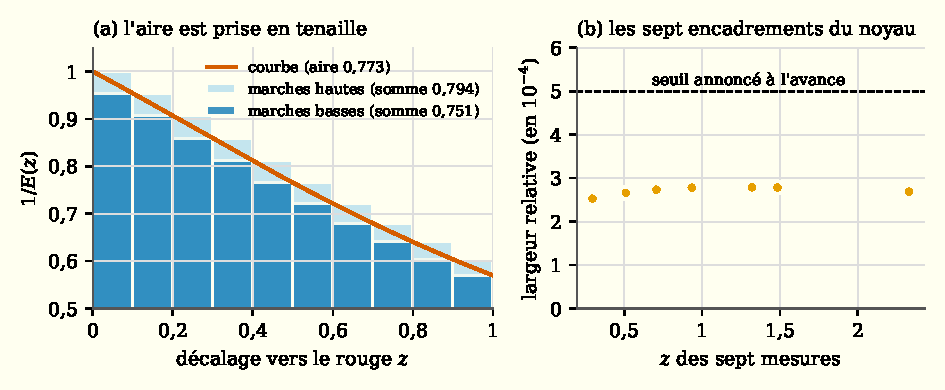
\includegraphics[width=\linewidth]{figures/c01_encadrement}
\caption{(a) Principe de la tenaille, sur 10 marches pour qu'on les voie (le calcul réel en utilise 2\,000 par unité
de $z$). (b) Largeur relative des sept encadrements vérifiés, lue dans les fractions exactes des théorèmes.}
\label{fig:c01}
\end{figure}

\section*{Comment on s'est assuré que ce n'est pas faux}

\niveau{As} \emph{Le juge a regardé, sans rejeu.} Le juge est ici Lean, un programme qui contrôle chaque pas logique
d'une preuve ; son cœur, le « noyau », a vérifié les tables d'entiers une à une, sans le raccourci qui ferait
confiance au compilateur. Les 55 théorèmes n'utilisent que les trois hypothèses de base admises partout. En revanche,
ces fichiers ne font pas partie du rejeu complet par un second programme de contrôle effectué le 26 octobre : d'où la
mention « sans rejeu ».

Cinq hypothèses avaient été écrites \emph{avant} de calculer. Quatre ont été confirmées, la cinquième (un encadrement
de la qualité d'ajustement) n'a pas été tentée. Des tests faits pour échouer ont bien échoué : une table d'entiers
falsifiée (une borne abaissée d'un million d'unités) a été rejetée par le noyau ; une fausse « preuve » laissée en
blanc et un axiome caché ont été signalés par l'audit. Un cas d'école dont la réponse est connue exactement (un univers
fait uniquement de matière) tombe bien dans son encadrement.

Un agent d'IA indépendant de celui qui a produit le travail a tout recompilé, ajouté ses propres pièges (rejetés),
recalculé chaque distance avec 50 chiffres exacts, et rendu un avis favorable assorti de corrections sur la portée des
affirmations. Comme tout ce livre, ce travail a été produit par des agents d'IA sous la direction de l'auteur et
audité par d'autres agents d'IA : aucun humain spécialiste ne l'a relu. Les valeurs des solveurs, elles, restent des
calculs ordinaires \niveau{X}.

\section*{Ce que ça ne dit pas}

\begin{limite}
\begin{itemize}
\item Une seule valeur de $\Omega_m$, celle du projet, et rien ne garantit que ce soit le meilleur ajustement.
\item Le modèle est imposé : univers plat, sans rayonnement. La machine ne dit pas si ce modèle est le bon.
\item Le passage aux grandeurs publiées par DESI et la comparaison avec leurs mesures sont faits hors de Lean.
\item Ce n'est pas une nouvelle mesure de l'univers : c'est un calcul de référence vérifié.
\item Le test des solveurs a la finesse de l'encadrement ($10^{-4}$) : un calcul à tolérance $10^{-3}$ passe aussi.
\end{itemize}
\end{limite}

\section*{Pour aller plus loin}

La même méthode, des certificats en nombres entiers relus par le noyau, a été réutilisée deux jours plus tard pour
toute la vraisemblance des données (chapitre suivant). Article et fichiers : doi:10.5281/zenodo.23247730.
